\documentclass[tikz]{standalone}
\usepackage{tikz}
\usetikzlibrary{patterns,snakes}
 
\begin{document}
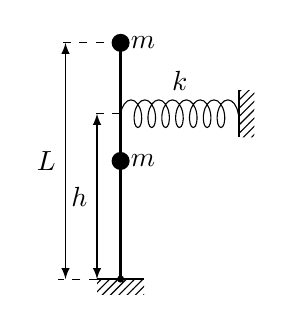
\begin{tikzpicture}
	\draw [very thick] (0,0) -- (0,3);
	\draw [snake=coil, segment amplitude=5pt, segment length=5pt] (0,2.1) -- (1.5, 2.1) node [midway, above=5pt] {$k$};
	\draw [thick] (1.5,2.4)--(1.5,1.8) (-0.3,0)--(0.3,0);
	\draw [draw=none, pattern=north east lines] (-0.3,0) rectangle (0.3,-0.2) 
											   (1.5,2.4) rectangle (1.7,1.8);
	\draw [thick, fill] (0, 0) circle (0.03);
	\draw [thick, fill] (0, 3) circle (0.1) node [right] {$m$};
	\draw [thick, fill] (0, 1.5) circle (0.1) node [right] {$m$};
	\draw [arrows={latex-latex}] (-0.3,0)--(-0.3,2.1) node [midway, left] {$h$};
	\draw [arrows={latex-latex}] (-0.7,0)--(-0.7,3) node [midway, left] {$L$};
	\draw [dashed] (-0.3,0) -- (-0.8,0) (0,2.1) -- (-0.4, 2.1) (0,3) --(-0.8,3);
\end{tikzpicture}
\end{document}